\documentclass{article}

\usepackage[letterpaper,margin=2.5cm]{geometry}
\usepackage{color}
\usepackage{amssymb}
\usepackage{amsmath}
\usepackage{libertine}
\usepackage{inconsolata}
\usepackage{euler}
\usepackage{graphicx}
\usepackage{framed}
\usepackage[colorlinks=true,linkcolor=blue,citecolor=red]{hyperref}
\usepackage[final]{microtype}
\usepackage{nameref}
\usepackage{todonotes}
\usepackage[nottoc,numbib]{tocbibind} % references in TOC
\usepackage{titletoc}

% Header configuration
\usepackage{fancyhdr}
\makeatletter
\rhead{\@currentlabelname}
\cfoot{}
\rfoot{\thepage}
\makeatother
\pagestyle{fancy}

\setlength{\parindent}{0mm}

\newcommand{\note}[1]{ %\
 \begin{framed} %\
 #1 %\
 \end{framed} }

\newcommand{\refdes}[1]{\texttt{#1}}
\newcommand{\mr}[1]{\ensuremath{\mathrm{#1}}}

\title{Owner's Manual}
\author{WCP52}

\begin{document}

\maketitle
\thispagestyle{empty}

\tableofcontents
\setlength{\parskip}{4mm}

\newpage
\section{Introduction}
\label{sec:intro}

\newpage
\section{Specifications}

\newpage
\section{Operating Information}

\newpage
\section{Theory of Operation}

This section contains a decription of the operation of the gain/phase analyzer.
Explanations start from the simple and broad, and descend to very specific
levels. It is expected that the reader has an understanding of the basics of
gain/phase analysis itself, which is explained in the \hyperref[sec:intro]{Introduction
section}.

\subsection{Block Diagram}

\begin{figure}[h]
\centering
\missingfigure[figwidth=3in]{Block diagram}
\caption{Block diagram}
\label{fig:blockdiagram}
\end{figure}

\subsection{Power Input Circuit}

\begin{figure}[h]
\centering
\missingfigure[figwidth=3in]{Power input circuit}
\caption{Power input circuit}
\label{fig:powerinput}
\end{figure}

This instrument is complex and has many somewhat expensive parts, so a full
input subsystem was designed to ensure that these parts are always supplied
correctly with power. This subsystem provides the following features:

\begin{itemize}
\item{Overcurrent protection}
\item{Reverse polarity protection}
\item{Undervoltage lockout}
\item{Overvoltage protection}
\item{Inrush current limiting}
\end{itemize}

The first piece of this input system, and possibly the simplest, is
\refdes{R81}. \refdes{R81} is a \emph{resettable fuse}, a type of resistor
with a positive temperature coefficient. Its resistance is very low
(around $0.5\;\Omega$) at room temperature.  As the current flowing through it
increases, it heats up, and as it heats up, its resistance increases.
Eventually, it will reach a point where this process `snowballs', and its
resistance is high enough that almost no current can flow through it. This
allows it to act like a fuse, but without permanently blowing: as soon as it
cools back down, it will conduct again.

\begin{figure}[h]
\centering
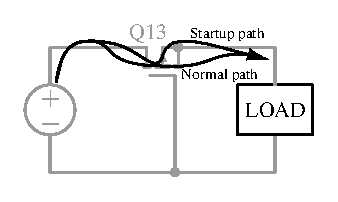
\includegraphics[width=3in]{mosrpp}
\caption{MOS reverse polarity protection circuit, simplified}
\label{fig:mosrpp}
\end{figure}

Once input current has passed through the resettable fuse, it encounters
\refdes{Q13}. A simplified form of this part of the circuit can be seen in
figure~\ref{fig:mosrpp}. Remember that a MOSFET has `parasitic' diodes
connected from the transistor's channel to its substrate; in a
standard power MOSFET, one ends up connected between the two ends of the
channel (the other ends up shorted to itself). In a P-channel MOSFET, this
diode points from the source to the drain. In this circuit, when power is
applied with the correct polarity, this diode allows current to initially take
the path labeled \emph{startup path}. When it does so, the voltage applied to
the load begins to rise, but the gate stays low, as it is tied to ground.
Eventually, the voltage rises high enough that the gate-source voltage switches
on the MOSFET, and current begins to flow through the \emph{normal path}
instead. This path takes the current through the low-impedance MOSFET channel,
rather than through the diode where the forward threshold voltage of the diode
would be lost.

If power is applied in the incorrect polarity, the substrate diode never
conducts, so the MOSFET never switches on.

After the reverse polarity protection, the current must flow through
\refdes{Q14}, which is connected as a traditional switch. \refdes{R88} holds
its gate and source together when the power is switched off, keeping the MOSFET
also turned off.

\begin{figure}[h]
\centering
\missingfigure[figwidth=3in]{Comparator circuit}
\caption{UVLO and OVLO circuit}
\label{fig:uovlo}
\end{figure}

To simplify things, the subcircuit in figure~\ref{fig:uovlo} is powered through
a simple diode for its own reverse-polarity protection. Bandgap voltage reference
\refdes{U11} does not need this, as its internal circuit has an antiparallel diode
built in~\cite{tl431}.

\refdes{U11} provides an accurate $2.5\;\mr{V}$ level against which the input
voltage can be compared.

\subsubsection{USB Power Input Circuit}

\subsection{Switching DC-DC Converters}

\subsection{Linear Regulators}

\subsection{Microcontroller}
\subsubsection{USB Communications}

\subsection{Synthesizer}

\subsection{Synthesizer Output Amplifiers}

\subsection{Output System}

\subsubsection{Attenuator and Filter}
\subsubsection{Gain Stages and Termination}

\subsection{Input System}

\subsubsection{Protection}
\subsubsection{Switching}
\subsubsection{Buffer and Filter}
\subsubsection{Logarithmic Detector}

\subsection{Signal Processing}
\subsubsection{Sampling}
\subsubsection{Null Search}
\subsubsection{Calibration}

\subsection{User Interface}

\newpage
\begin{thebibliography}{9}
\bibitem{tl431}
Texas Instruments, ``TL43xx Precision Programmable Reference,''
TL431 datasheet, Aug. 2004 [Revised Jan. 2015].
\end{thebibliography}

\end{document}
